\documentclass[a4paper,12pt]{article}

% Module de base utf, français
\usepackage[utf8]{inputenc}
\usepackage[T1]{fontenc}
\usepackage[french]{babel}
% gestion des marges
\usepackage[top=2cm, bottom=2cm, left=2cm, right=2cm]{geometry}

% quote
% \usepackage{csquotes}

% Packages math
%\usepackage{amsmath}
%\usepackage{amssymb}
%\usepackage{mathrsfs}

% Package tableau
\usepackage{multirow}

% Package insertion d'image
\usepackage{graphicx}
\usepackage{float}
\usepackage{subcaption} %image multiple

% Package url
\usepackage{url}	

% Package de couleur
\usepackage{color}
\usepackage[colorlinks,linkcolor=black,urlcolor=blue]{hyperref}

% Package pour le code, nécessite package color
\usepackage{listings}
\usepackage{amsmath}
\lstset{ % General setup for the package
	language=Python,
	basicstyle=\small\sffamily,
	numbers=left,
 	numberstyle=\tiny,
	frame=tb,
	tabsize=4,
	columns=fixed,
	showstringspaces=false,
	showtabs=false,
	keepspaces,
	commentstyle=\color{red},
	keywordstyle=\color{blue},
	breaklines=true
}

% Packages Verbatim
%\usepackage{moreverb}

% nouvelle commande pour ~
%\newcommand{\tidle}{\char`\~}

\title{Projet L3\\Ingénierie des langues\\Fouille de données}
\author{GOEHRY Martial\\16711476}

\begin{document}
	\maketitle
	\tableofcontents
	\newpage
	
\section{Introduction}
	Ce projet a pour but de développer un modèle permettant de catégoriser des emails en spam ou ham.
	La définition d'un spam dans le dictionnaire \emph{Larousse} est:
	
	\begin{quote}
	"Courrier électronique non sollicité envoyé en grand nombre à des boîtes aux lettres électroniques ou à des forums, dans un but publicitaire ou commercial."
	\end{quote}
	
	Il est possible d'ajouter à cette catégorie tous les mails indésirables comme les tentatives d'hameçonnage permettant de soutirer des informations personnelles à une cible.\\ 
	
	L'objectif est de travailler uniquement sur les données textuelles issues du corps du mail.
	Nous avons donc en point de départ les éléments suivants:
	\begin{itemize}
		\item langue: anglais
		\item corpus: monolingue écrit
		\item type: e-mail
	\end{itemize}
	
	\paragraph{Déroulé} Le développement de ce projet s'articule autour de 3 phases majeurs
		\begin{itemize}
			\item Phase 1 : Récupération des données
			\item Phase 2 : Analyse des caractéristiques
			\item Phase 3 : Construction du modèle
		\end{itemize}
		
	
	\subparagraph{Phase 1} La phase 1 concerne la récolte des informations et les traitements minimums nécessaires pour la mise en base. Les objectifs de traitement de cette phase sont:
	\begin{itemize}
		\item Extraire les corps des mails et éliminer les méta-données superflues
		\item Eliminer les mails non anglais
		\item Eliminer les mails en doublons
		\item Eliminer les parties de textes non pertinente (liens, réponses, certaines ponctuations)
	\end{itemize}
	Cette phase se termine avec la mise en base des documents dans un index ElasticSearch.
	
	\subparagraph{Phase 2} La phase 2 vise à générer les données statistiques et numériques à partir des corps de mails. Lors de cette phase une analyse statistique manuelle des données est réalisée
	% todo : description rapide des actions de la phase 2
	
	\subparagraph{Phase 3} La phase 3 regroupe tous les opérations d'exploitation des données et vise à développer et à créer un modèle de classement des mails et d'en évaluer les performances.\\
	
	Afin de conserver une certaine cohérence dans le déroulé entre les phases et au vu du temps que j'ai pris pour réaliser ce projet l'ensemble des étapes est automatisé en langage Python. Seule la récolte initiale des mails a été réalisée à la main.\\
	
	Le schéma ci-dessous donne une vue synthétique des étapes du projet
	\begin{figure}[H]
		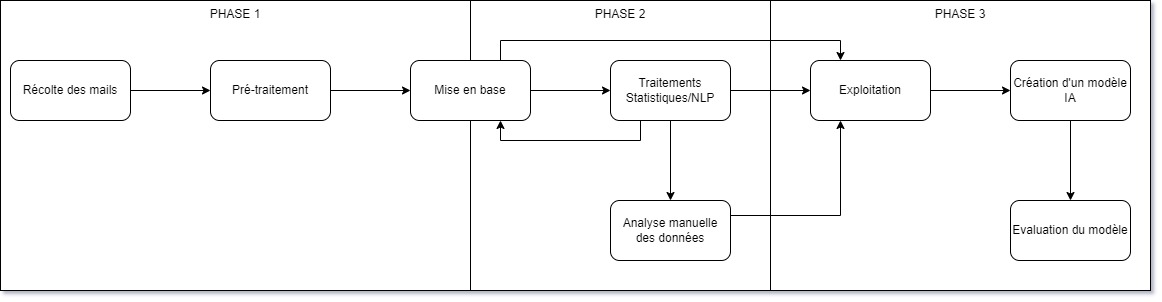
\includegraphics[width=\linewidth]{img/SchemaGeneral.jpg}
		\caption{Schéma des grandes étapes}
	\end{figure}
		 
\newpage

\section{Phase 1 : Récupération des données}
	La phase 1 est une pipeline qui vas permettre d'extraire un maximum d'information d'un email en essayant de pas dénaturer le fond ni la forme. Il pourra ensuite être stocké avec sa catégorie d'appartenance. Durant cette phase nous allons également initialiser les bases de données en créant les index (ES) et les tables (PSQL et SQLITE). 
	
	Ci-dessous le schéma général de cette phase.
	\begin{figure}[H]
		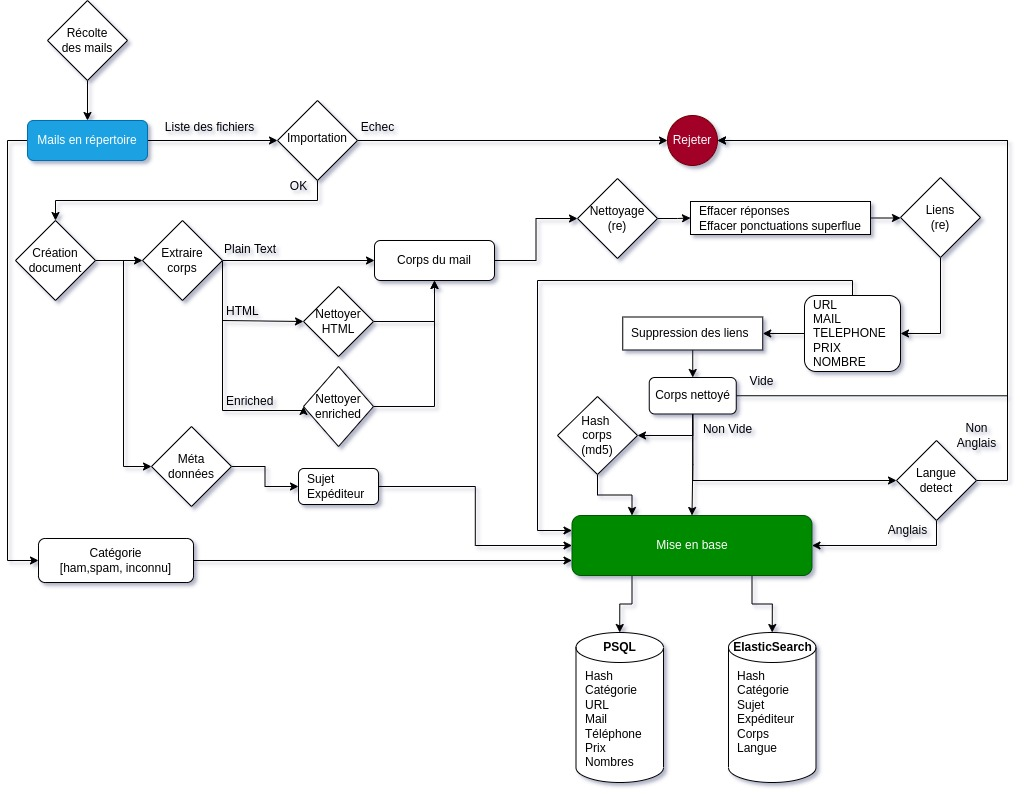
\includegraphics[width=\linewidth]{img/SchemaPhase1.jpg}
		\caption{Schéma des étapes de la phase 1}
	\end{figure}


	\subsection{Récolte des données}
		\paragraph{Recherche de dataset}
			J'avais dans l'idée de faire la recherche de mails en français. Cependant, je n'ai pas trouvé de dataset dans cette langue. Je me suis donc retourné vers les datasets de mails en anglais. \\
			J'ai pu alors récupérer deux dataset:
			\begin{itemize}
				\item Enron company mails (voir: \ref{Enron_dataset})
				\item Dataset SpamAssassin (voir: \ref{SpamAssassin_dataset})
			\end{itemize}
			Les mails de SpamAssassin ont l'avantage d'être pré-trié, contrairement aux mails de la compagnie Enron. Ainsi le développement du moteur se fera uniquement avec les mails du SpamAssasin afin de pouvoir vérifier les résultats de l'analyse. 
		
		\paragraph{Téléchargement des données}
			Le téléchargement du dataset Enron est possible a partir du moment où l'on possède un compte sur la plateforme Kaggle. Le dataset SpamAssassin est ouvert, il suffit de télécharger les archives de chaque catégorie. \\
			
			La récolte des données a été réalisée à la main sans automatisation. 
			Les mails sont alors stockés dans plusieurs répertoires \emph{HAM} et \emph{SPAM} selon leur catégorie. \\
			
			Format:
			\begin{itemize}
				\item \emph{Enron} - 1 fichier CSV avec tous les mails
				\item \emph{SpamAssassin} - 1 fichier texte par mail
			\end{itemize}
	
	\subsection{Pré-traitement}
		Les étapes de pré-traitement regroupent toutes les étapes et actions réalisées avant la mise en base. 
		L'objectif de ces étapes est d'extraire le message en retirant les métadonnées du mail.
		Il va être possible d'effectuer certain traitement de nettoyage et de récupération d'informations sommaires.
		
		Les manipulations de messages dans Python se font principalement à l'aide du module \emph{email} natif. 
		
		\subsubsection{Importation}		
			La fonction \emph{email.message\_from\_binary\_file} permet de transformer un fichier mail en objet python manipulable :
			\begin{lstlisting}[title=Fonction d'importation des fichiers]
def import_from_file(chemin):
    try:
        with open(chemin, 'rb') as data:
            msg = message_from_binary_file(data, policy=policy.default)
            return msg
	
    except FileNotFoundError:
        print("Fichier : '{}' non trouve".format(chemin), file=sys.stderr)
        return None\end{lstlisting}
		
		
		\subsubsection{Extraction des corps des mails}
			Une fois le fichier importé au format \emph{EmailMessage}, il est possible d'en extraire le corps.
			
			Le corps du mail peut être composé de plusieurs parties qui ne sont pas forcément du texte. Les parties non textuelles ne sont pas conservée. 
					
		    	\begin{lstlisting}[title=Extraction du corps du mail]
def extract_body(msg):
    refused_charset = ['unknown-8bit', 'default', 'default_charset',
                       'gb2312_charset', 'chinesebig5', 'big5']
    body = ""

    if msg.is_multipart():
        for part in msg.walk():
            if not part.is_multipart():
                body += extract_body(part)
        return body

    if msg.get_content_maintype() != 'text':
        return ""

    if msg.get_content_charset() in refused_charset:
        return ""

    if msg.get_content_subtype() == 'plain':
        payload = msg.get_payload(decode=True)
        body += payload.decode(errors='ignore')

    if msg.get_content_subtype() == 'html':
        payload = msg.get_payload(decode=True)
        body += nettoyage.clear_html(payload.decode(errors='ignore'))

    if msg.get_content_subtype() == 'enriched':
        payload = msg.get_payload(decode=True)
        body += nettoyage.clear_enriched(payload.decode(errors='ignore'))

    return body \end{lstlisting}
	    		
		\subsubsection{Nettoyage}
			Le nettoyage du texte utilise principalement les expressions régulières pour retirer un maximum d'éléments indésirables dans le texte. J'utilise 2 modules externes afin de traiter le code HTML et faire la détection des mails qui ne sont pas écrit en anglais.
			
			\paragraph{Par regex} J'utilise le module python \emph{re} pour générer les suivantes:
				\subparagraph{Suppression des réponses} Lorsque l'on réponds à un mail, le texte du message précédent est conservé dans le corps du mail. Afin de permettre la distinction avec les mails précédent le caractère '>' est ajouter en début de ligne. Je retire toutes les lignes correspondant à des réponses afin de limiter les doublons.
				
					\begin{lstlisting}[title=Nettoyage des réponses]
def clear_reply(texte):
    pattern = re.compile('^>.*$', flags=re.MULTILINE)
    return re.sub(pattern, '', texte) \end{lstlisting}
					
				\subparagraph{Suppression des ponctuations} Afin de ne pas surcharger la base de données et pour se concentrer sur le texte, une grande partie des caractères de ponctuation seront retirés. L'idée est de se concentrer sur les ponctuations les plus présentes (.,?!) 

					\begin{lstlisting}[title=Nettoyage des ponctuations]				
def clear_ponctuation(texte):
    pattern_ponct = re.compile('[*#\\-_=:;<>\\[\\]"\'~)(|/$+}{@%&\\\]', flags=re.MULTILINE)
    return re.sub(pattern_ponct, ' ', texte) \end{lstlisting}

				% Suppression des balises pour les enriched text
				\subparagraph{Suppression des balises pour les enriched text} Certaines parties du corps de mail sont de type \emph{enriched text}. Les balises ne sont pas pertinente dans notre analyse et sont donc retirées.
						
					\begin{lstlisting}[title=Nettoyage des balises enriched text]
def clear_enriched(texte):
    pattern = re.compile('<.*>')
    return re.sub(pattern, '', texte) \end{lstlisting}
						
				% Modification des liens (URL, MAIL et TELEPHONE)
				\subparagraph{Suppression des liens} Certaines informations présentent dans le texte ne peuvent pas être utilisées dans l'analyse textuelle. Cependant il peut être intéressant de conserver une trace de leur présence. Nous allons donc modifier les liens url, mail et les numéros de téléphone qui seront comptabilisé avant d'être retiré du texte.
				
					\begin{lstlisting}[title=Nettoyage des liens]
def change_lien(texte, liens):
    pattern_mail = re.compile('[a-zA-Z0-9_.+-]+@[a-zA-Z0-9-]+\\.[a-zA-Z0-9-.]+')

    pattern_url1 = re.compile('(http|ftp|https)?:\/\/([\w\-_]+(?:(?:\.[\w\-_]+)+))'
                             '([\w\-\.,@?^=%&:/~\+#]*[\w\-\@?^=%&/~\+#])?', flags=re.MULTILINE)
    pattern_url2 = re.compile('(\\w+\\.)+\\w+', flags=re.MULTILINE)
    pattern_tel1 = re.compile('\\(\\d{3}\\)\\d+-\\d+')  # (359)1234-1000
    pattern_tel2 = re.compile('\\+\\d+([ .-]?\\d)+')    # +34 936 00 23 23

    temp, liens['MAIL'] = re.subn(pattern_mail, ' ', texte)

    temp, liens['URL'] = re.subn(pattern_url1, ' ', temp)
    temp, nb = re.subn(pattern_url2, ' ', temp)
    liens['URL'] += nb

    temp, liens['TEL'] = re.subn(pattern_tel1, ' ', temp)
    temp, nb = re.subn(pattern_tel2, ' ', temp)
    liens['TEL'] += nb

    return temp \end{lstlisting}
 
 
				% Modification des nombes (NOMBRE et PRIX)
				\subparagraph{Suppression des nombres} Comme pour les liens, les nombres sont comptabilisés et retirés. Je fais la distinction entre les nombres seuls et les nombres accompagnés de sigle monétaires. 
				
				\begin{verbatim}
monnaie = '€$£'
				\end{verbatim}
					\begin{lstlisting}[title=Nettoyage des nombres]
def change_nombres(texte, liens):
    pattern_prix1 = re.compile(f'[{monnaie}]( )?\\d+([.,]\\d+)? ', flags=re.MULTILINE)
    pattern_prix2 = re.compile(f' \\d+([.,]\\d+)?( )?[{monnaie}]', flags=re.MULTILINE)
    pattern_nb = re.compile('\\d+')

    temp, liens['PRIX'] = re.subn(pattern_prix1, ' ', texte)
    temp, nb = re.subn(pattern_prix2, ' ', temp)
    liens['PRIX'] += nb

    temp, liens['NOMBRE'] = re.subn(pattern_nb, ' ', temp)

    return temp \end{lstlisting}
 
 
			\paragraph{Par module}
				J'ai utilisé deux modules externes plus performant que ce que j'aurais pu faire avec simplement des expressions régulières. 
				
				% Suppression balise HTML avec BeautifulSoup
				\subparagraph{Suppression du code HTML} Certaines parties du corps du mail sont de type HTML. J'utilise le module \emph{BeautifulSoup} pour parser le code et récupérer le texte affiché. 
		
					\begin{lstlisting}[title=Nettoyage des nombres]		
from bs4 import BeautifulSoup

def clear_html(texte):
    brut = BeautifulSoup(texte, "lxml").text
    return brut \end{lstlisting}	
    		
				% Retrait des mails en langue non anglaise
				\subparagraph{Sélection des mails en anglais} Lors de mes tests, je me suis rendu compte que certains mails n'étaient pas en anglais. J'ai donc trouvé le module \emph{langdetect} qui permet de détecter le langage utilisé dans un texte en utilisant un modèle Naïve Bayes avec une précision de 99\% (voir \ref{langdetect}). \\
				Je conserve dans les données à mettre en base le langage détecté dans l'idée de pouvoir traité plusieurs langues (en idée d'évolution).\\
				
				La détection de la langue se fait dans la fonction s'occupant de créer le document pour la mise en base ElasticSearch.
				
				\begin{lstlisting}[title=Création d'un document]	
import langdetect

def create_document(mail, categorie):
    corp = mail_load.extract_body(mail)
    corp, liens = nettoyage.clear_texte_init(corp)
    sujet, expediteur = mail_load.extract_meta(mail)

    if not corp:
        return None

    try:
        lang = langdetect.detect(corp)
    except langdetect.lang_detect_exception.LangDetectException:
        return None

    if lang != 'en':
        return None

    if categorie.lower() not in ['spam', 'ham']:
        categorie = 'inconnu'

    doc = {
        'hash': hashlib.md5(corp.encode()).hexdigest(),
        'categorie': categorie.lower(),
        'sujet': sujet,
        'expediteur': expediteur,
        'message': corp,
        'langue': lang,
        'liens': liens
    }
    return doc \end{lstlisting}
 
 
			\paragraph{Exemple de traitement}
				Les sections suivantes présentent des exemples de traitement de la phase 1.
				
				\begin{lstlisting}[title=Traitement initial]
message = '''
Message dedicated to be a sample to show how the process is clearing the text.

Begin reply :
> He once said
>>> that it would be great
End of reply.

Substitutions :
spamassassin-talk@example.sourceforge.net
https://www.inphonic.com/r.asp?r=sourceforge1&refcode1=vs3390
hello.foo.bar
between $ 25 and 25,21 $

A number is : 2588,8 588
Phone type a : (359)1234-1000
Phone type b : +34 936 00 23 23
Ponctuation : ----## ..
~ ~~~~~
'''
text, liens = clear_texte_init(message)
print(liens)
print(text) 
				\end{lstlisting}

				Résultat traitement initial :
				\begin{verbatim}
{'URL': 2, 'MAIL': 1, 'TEL': 2, 'NOMBRE': 3, 'PRIX': 2}

Message dedicated to be a sample to show how the process is clearing the text.

Begin reply 


End of reply.

Substitutions 



between and

A number is  , 
Phone type a  
Phone type b  
Ponctuation   ..
				\end{verbatim}
				
				\begin{lstlisting}[title=Traitement HTML]
message_html = '''
<!DOCTYPE html PUBLIC "-//W3C//DTD HTML 4.01 Transitional//EN">
<html>
<head>
  <title>Foobar</title>
</head>
<body>
I actually thought of this kind of active chat at AOL 
bringing up ads based on what was being discussed and 
other features
  <pre wrap="">On 10/2/02 12:00 PM, "Mr. FoRK" 
  <a class="moz-txt-link-rfc2396E"href="mailto:fork_
  list@hotmail.com">&lt;fork_list@hotmail.com&gt;</a> 
  wrote: Hello There, General Kenobi !?
<br>
</body>
</html>
'''
print(clear_html(message_html))
				\end{lstlisting}
				Résultat traitement HTML :
				\begin{verbatim}

Foobar


I actually thought of this kind of active chat at AOL 
bringing up ads based on what was being discussed and 
other features
  On 10/2/02 12:00 PM, "Mr. FoRK" 
  <fork_list@hotmail.com> 
  wrote: Hello There, General Kenobi !?


				\end{verbatim}

				\begin{lstlisting}[title=Traitement enriched text]
message_enriched = '''
<smaller>I'd like to swap with someone also using Simple DNS to take
advantage of the trusted zone file transfer option.</smaller>
'''
print(clear_enriched(message_enriched))
				\end{lstlisting}
				Résultat traitement enriched text :
				\begin{verbatim}
I'd like to swap with someone also using Simple DNS to take
advantage of the trusted zone file transfer option.
				\end{verbatim}


		\subsubsection{Mise en base}
		
			\begin{figure}[H]
				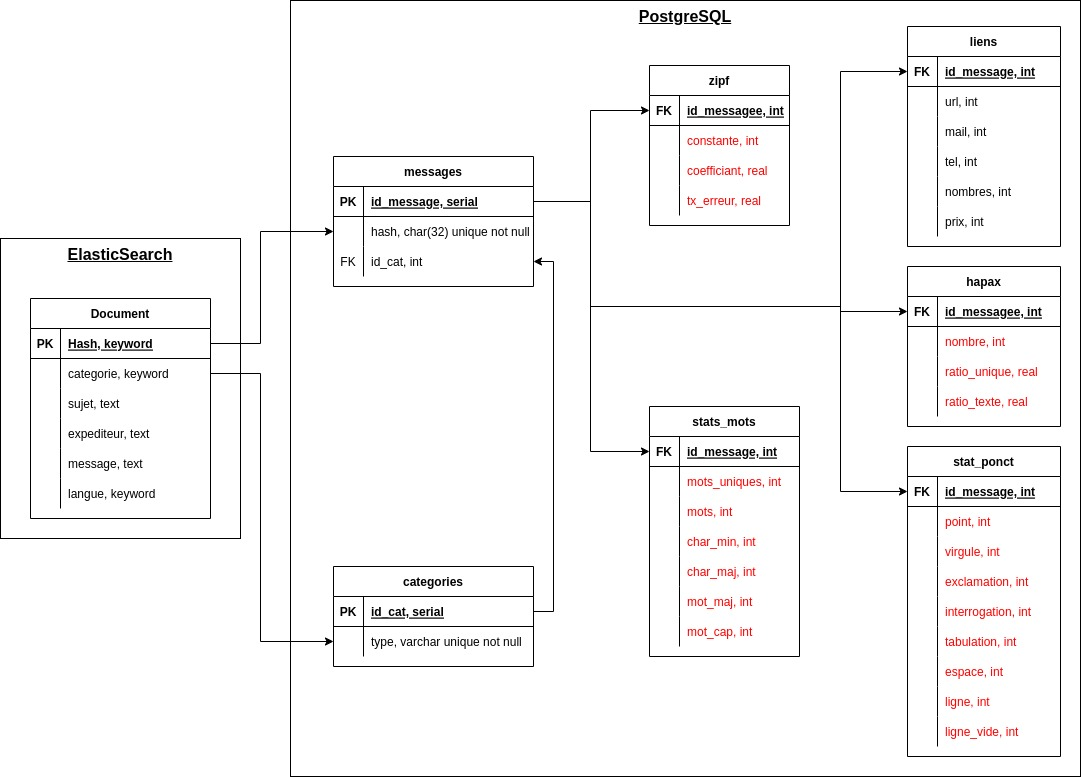
\includegraphics[width=\linewidth]{img/SchemaBdd.jpg}
				\caption{Schéma des bases de données de l'application}
			\end{figure}
		
			\paragraph{Stockage des données: ElasticSearch}
				% fonction de hashage
								
			\paragraph{Stockage des premières informations statistiques: PostgreSQL}
			
			\paragraph{Stockage des données statistiques du traitement: SQLite}
				% Informations pour la soutenance
				\begin{figure}[H]
					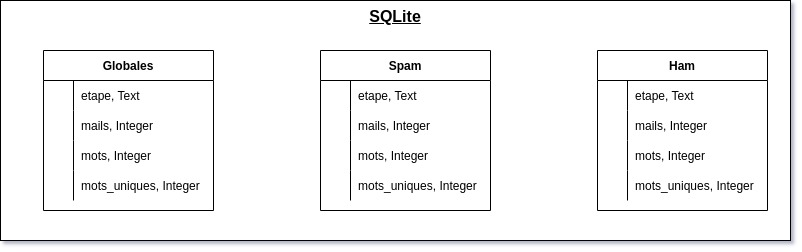
\includegraphics[width=\linewidth]{img/Schemasqlite.jpg}
					\caption{Schéma de la base de données pour lors du traitement}
				\end{figure}
				
			
			
	
	\subsection{Données de la phase 1}
		
	
\newpage
\section{Phase 2}
	\subsection{Traitement}
	
		\subsubsection{Recherche de caractéristiques}
			\paragraph{Références}
				% LIENS, Nombres
							
				
		\subsubsection{Analyse préliminaire}
			% Etudes statistiques
			% Etudes des distributions
			% Travail sur la distribution de zipf

\newpage
\section{Phase 3}

\newpage	
\appendix
\section{Développement visualisation distribution de Zipf}
	\paragraph{Présentation}
		La loi de distribution de Zipf est une loi empirique (basée sur l'observation) qui veut que le mot le plus fréquent est, à peu de chose près, 2 fois plus fréquent que le $2^{eme}$, 3 fois plus fréquent que le $3^{eme}$ etc.\\
		
		La formulation finale de la $1^{ere}$ loi de Zipf est la suivante :
		
		\begin{align*}
				|mot| = constante \times rang(mot)^{k \approx 1}
		\end{align*}
		
		avec \emph{$|mot|$} la fréquence d'apparition d'un mot, \emph{constante} une valeur propre à chaque texte, \emph{rang(mot)} la place du mot dans le tri décroissant par fréquence d'apparition et \emph{k} un coefficient proche de 1. 
		
	\paragraph{Développement}
		Afin de pouvoir utiliser les résultats de cette distribution dans mon analyse, j'ai développé un ensemble de fonctions sur un corpus "\emph{reconnu}". Mon choix s'est porté sur le corpus \emph{Brown} (voir \ref{Brown_corpus}) présent dans la librairie \emph{nltk}. Ce corpus contient environ 500 documents contenant 1 millions de mot en anglais.\\
		
		Le processus d'analyse se fait sur 2 versions de ce corpus.
		\begin{itemize}
			\item la première version contient tous les mots sans modifications
			\item le seconde version contient tous les mots sans les \emph{stopwords}
		\end{itemize}
		Les \emph{stopwords} sont des mots qui n'ont pas ou peu de signification dans un texte. Ces mots sont retirés dans la $2^e$ version pour voir l'effet d'une réduction sur la distribution de Zipf. \\
		
		Les paragraphes ci-dessous détaillent les étapes du développement :
		
		\subparagraph{Étape 1 - Ordonner les mots}
			La première étape est de compter les occurrences de tous les mots des 2 corpus et de les ranger en fonction de leur nombre d’occurrence. 
			\begin{lstlisting}[title=Triage des mots]
def frequence_mot(bag, freq=None):
    """
    Calcule la frequence de chaque mot dans un sac de mot
    :param bag: <list> - liste de tous les mots d'un texte
    :param freq: <dict> - dictionnaire avec {<str> mot: <int> frequence}
    :return: <dict> - dictionnaire avec la frequence par mot {mot: frequence}
    """
    if freq is None:
        freq = {}
    for mot in bag:
        freq[mot] = freq.get(mot, 0) + 1
    return freq
		
def classement_zipf(dico):
    """
    Trie un dictionnaire de mots : occurence et leur assigne un rang en fonction du nombre d'occurence
    :param dico: <dict> dictionnaire de mot: occurences
    :return: <list> {"rang": <int>, "mot": <str>, "frequence": <int>}
    """
    ranked = []
    for rang, couple in enumerate(sorted(dico.items(), key=lambda item: item[1], reverse=True), start=1):
        ranked.append({"rang": rang,
                       "mot": couple[0],
                       "frequence": couple[1]})

    return ranked \end{lstlisting}
    
    		
    		On obtient les représentations suivantes: 
		\begin{figure}[H]
				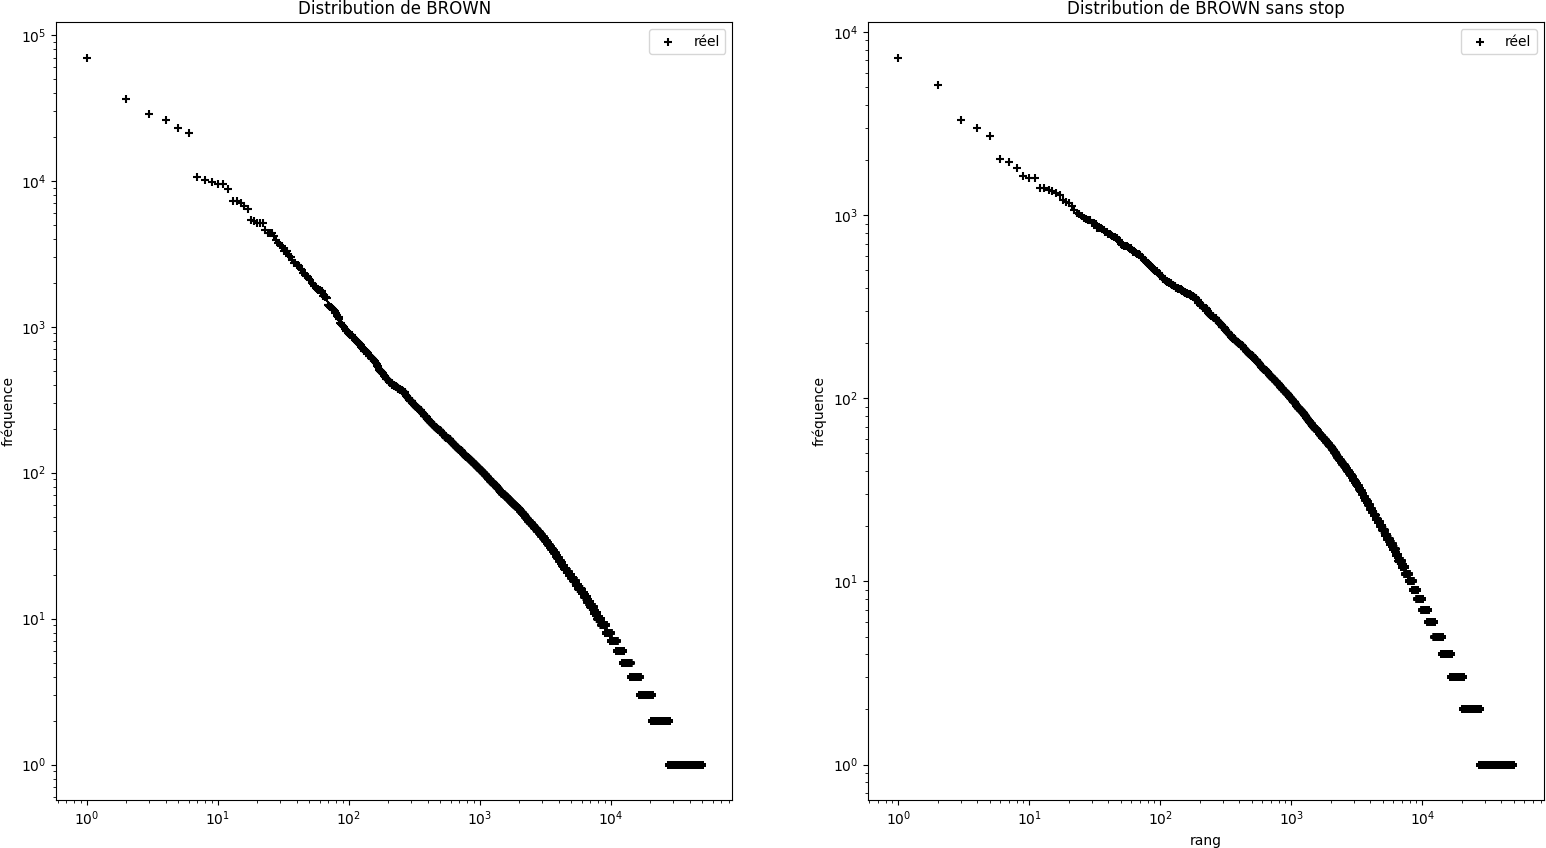
\includegraphics[width=\linewidth]{img/distribZipf.png}
				\caption{Distribution de Zipf pour les deux corpus}
			\end{figure}    		
    		
    		\begin{itemize}
    			\item Nombre de mots dans brown:	mots: 49398	occurences: 1012528
    			\item Nombre de mots dans brown stop:	mots: 49383	occurences: 578837\\
    		\end{itemize}
    		
    		La distribution de la version complète du corpus semble à première vue plus fidèle à la représentation classique de la distribution de Zipf. 
			
		\subparagraph{Etape 2 - calcul de la constante}
			Le premier paramètre que je détermine est la \emph{constante}. Pour ce faire j'effectue le calcul suivant pour tous les mots :
			
			\begin{align*}
				constante = |mot| \times rang(mot)
			\end{align*}
			
			On obtient une liste de toutes les constantes théoriques pour chaque mot selon son rang.
			De cette liste, nous allons extraire la moyenne et la médiane.
			
			\begin{figure}[H]
				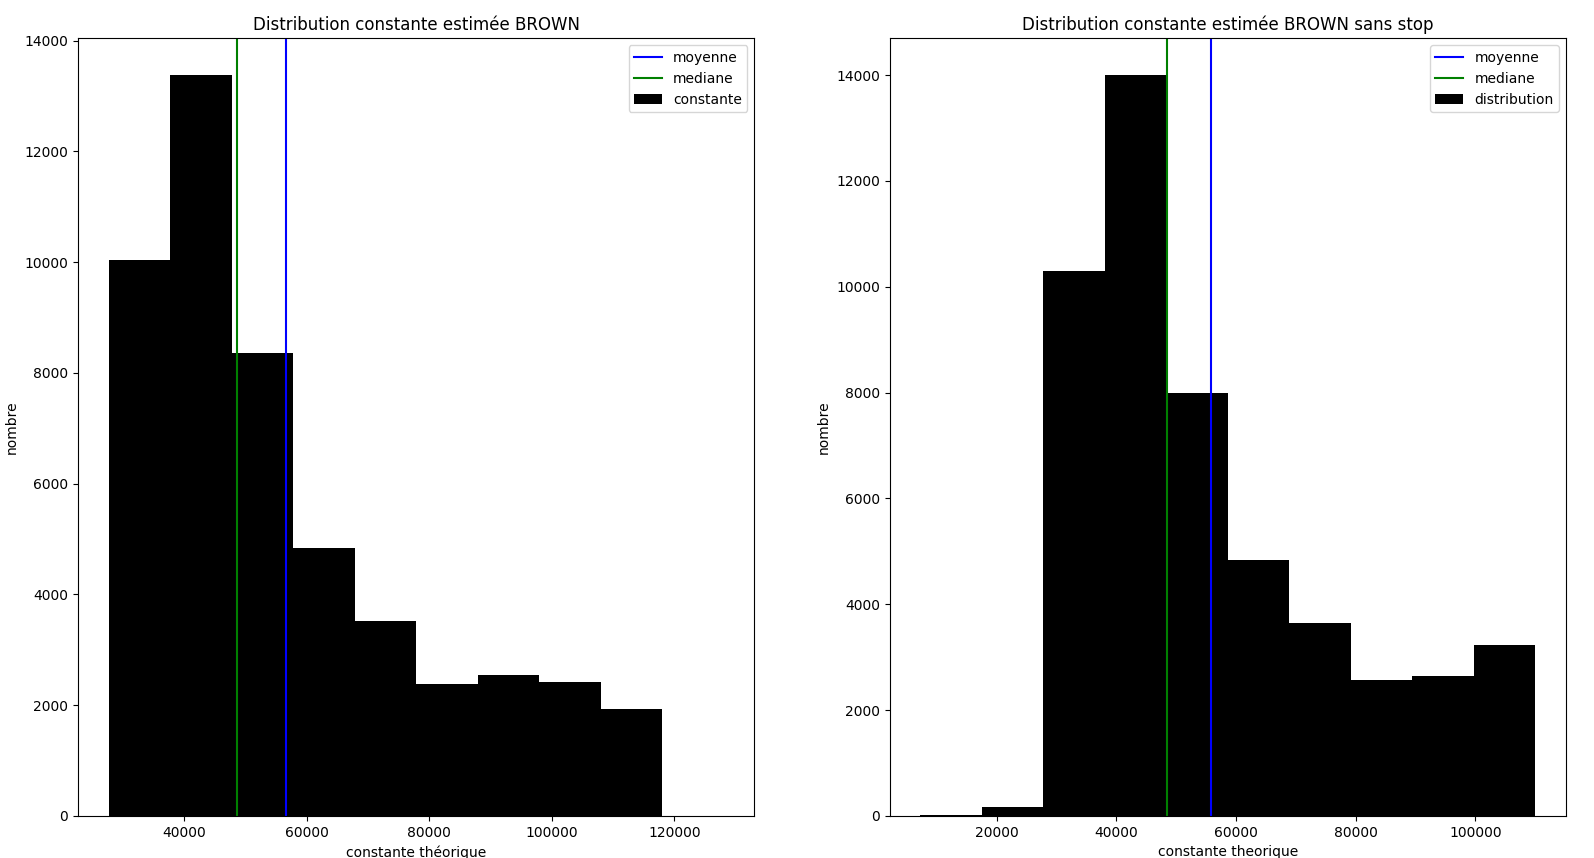
\includegraphics[width=\linewidth]{img/distribContTh.png}
				\caption{Distribution des constantes théoriques pour les deux corpus}
			\end{figure}
			
			On voit qu'il y a une majorité de mots donnent une constante brute comprise entre $20.000$ et $60.000$. Dans les deux corpus
			La différence entre les moyennes et médianes des deux corpus n'est pas flagrante :
			\begin{itemize}
				\item Brown moyenne: 56525.81, médiane: 48601.50
				\item Brown (- stopwords) moyenne: 55809.97, médiane: 48494.00
			\end{itemize}


		\subparagraph{Etape 3 - recherche du coefficient}
			Le coefficient $k$ permet d'ajuster le résultat, et pourra éventuellement donner une indication de complexité. La recherche de $k$ se fera sur les deux corpus avec utilisant les moyennes et médianes.\\
			
			Pour ce faire nous allons:

			\begin{enumerate}
				\item Faire la liste de tous les coefficients possibles dans l'intervalle $[0.86, 1.3]$ avec un pas de $0.01$\footnote{Borne et pas, totalement arbitraire afin d'obtenir un graphique présentable}.
				\item Calculer toutes la fréquences théoriques de tous les rangs avec tous les coefficients possibles avec en constante la moyenne et la médiane de chaque corpus.
				\item Calculer la moyenne des coûts absolus entre les fréquences théoriques par coefficient avec la fréquence réelle observée pour chaque corpus.\\
			\end{enumerate}
			
			Le couple coefficient/constante avec le coup minimal sera retenu pour l'utilisation dans la phase de \emph{feature engineering}. \\	
			
			\begin{lstlisting}[title=Fonctions utilisées dans la recherche du coefficient]
def zipf_freq_theorique(constante, rang, coef):
    """
    Calcul la frequence theorique d'un mot selon son rang, la constante du texte et un coeficiant d'ajustement
    :param constante: <int> constante determinee par la distribution de Zipf
    :param rang: <int> rang du mot selon sa frequence
    :param coef: <float> variable d'ajustement
    :return: <float> frequence theorique zipfienne
    """
    return constante / (rang ** coef)
    
def cout(l1, l2, methode):
    """
    Calcul le cout de l'ecart entre les elements de l1 et le l2, place par place
    :param l1: <list> liste d'entier
    :param l2: <liste> liste d'entier
    :param methode: <str> methode de calcul du cout
    :return: <float> cout selon methode
    """
    if len(l1) != len(l2):
        print("Erreur, fonction cout: l1 & l2 de taille differente", file=sys.stderr)
        return None

    if len(l1) == 0:
        print("Erreur, fonction cout: liste vide", file=sys.stderr)

    if methode.lower() not in ['absolue', 'carre', 'racine']:
        print("Erreur, fonction cout - methode '{}' inconnue".format(methode), file=sys.stderr)
        return None

    if methode.lower() == 'absolue':
        return np.mean([abs(x-y) for x, y in zip(l1, l2)])

    if methode.lower() == 'carre':
        return np.mean([(x-y)**2 for x, y in zip(l1, l2)])

    if methode.lower() == 'racine':
        return np.sqrt(np.mean([(x-y)**2 for x, y in zip(l1, l2)]))

    return None\end{lstlisting}

			\begin{lstlisting}[title=Calcul des fréquences par coefficient]
    ls_coef = list(np.arange(0.86, 1.3, 0.01))
    zbmo_th = {coef: [stats.zipf_freq_theorique(zb_const_moyen, r, coef) for r in zb_rang] for coef in ls_coef}
    zbme_th = {coef: [stats.zipf_freq_theorique(zb_const_median, r, coef) for r in zb_rang] for coef in ls_coef}
    zbmoth_cmoy = [stats.cout(zb_freq, zbmo_th[coef], 'absolue') for coef in ls_coef]
    zbmeth_cmoy = [stats.cout(zb_freq, zbme_th[coef], 'absolue') for coef in ls_coef]

    zbsmo_th = {coef: [stats.zipf_freq_theorique(zbs_const_moyen, r, coef) for r in zbs_rang] for coef in ls_coef}
    zbsme_th = {coef: [stats.zipf_freq_theorique(zbs_const_median, r, coef) for r in zbs_rang] for coef in ls_coef}
    zbsmoth_cmoy = [stats.cout(zbs_freq, zbsmo_th[coef], 'absolue') for coef in ls_coef]
    zbsmeth_cmoy = [stats.cout(zbs_freq, zbsme_th[coef], 'absolue') for coef in ls_coef] \end{lstlisting}
		
		La recherche du coefficient nous retourne les éléments suivants:
			\begin{figure}[H]
				\includegraphics[width=\linewidth]{img/coutZipf.png}
				\caption{Coût absolu moyen par coefficient}
			\end{figure}
		
			\begin{itemize}
				\item Coût min brown moyenne: 5.93, median: 7.01
				\item Coût min brown (- stopwords) moyenne: 6.95, median: 6.46
				\item Coefficient min brown moyenne: 0.92, median: 0.91
				\item Coefficient min brown (- stopwords) moyenne: 0.97, median: 0.95
			\end{itemize}
				
	\paragraph{Résultats}
		
		Le tableaux ci dessous rappelle les données récupérées au long de la recherche:
		\begin{center}
			\begin{tabular}{|l|c|c|}
				\hline
				& BROWN avec stopwords & BROWN sans stopwords \\
				\hline
				nombre de mots uniques & 49398 & 49383 \\
				\hline
				nombre de mots total & 1012528 & 578837 \\
				\hline
				Constante moyenne & 56525.81 & 55809.97 \\
				\hline
				Constante médiane & 48601.50 & 48494.00 \\
				\hline
				Coefficient avec moyenne & 0.92 & 0.97 \\
				\hline
				Cout du coefficient moyenne & 5.93 & 6.95 \\
				\hline
				Coefficient avec médiane & 0.91 & 0.95 \\
				\hline
				Cout du coefficient médiane & 7.01  & 6.46 \\
				\hline
			\end{tabular}		
		\end{center}
		
		D'après les données il est possible de dire que l'on obtient de meilleurs résultats si on conserve tous les mots du corpus. Dans ce cas l'utilisation de la moyenne des constantes génère un taux d'erreur plus faible que la médiane.\\
		
		Ci-dessous la représentation des fréquences théoriques avec le coefficient optimal pour chaque corpus et chaque méthode. On voit que la courbe de la constante moyenne sur le corpus brute est celle qui suit le mieux les données réelles.
		\begin{figure}[H]
			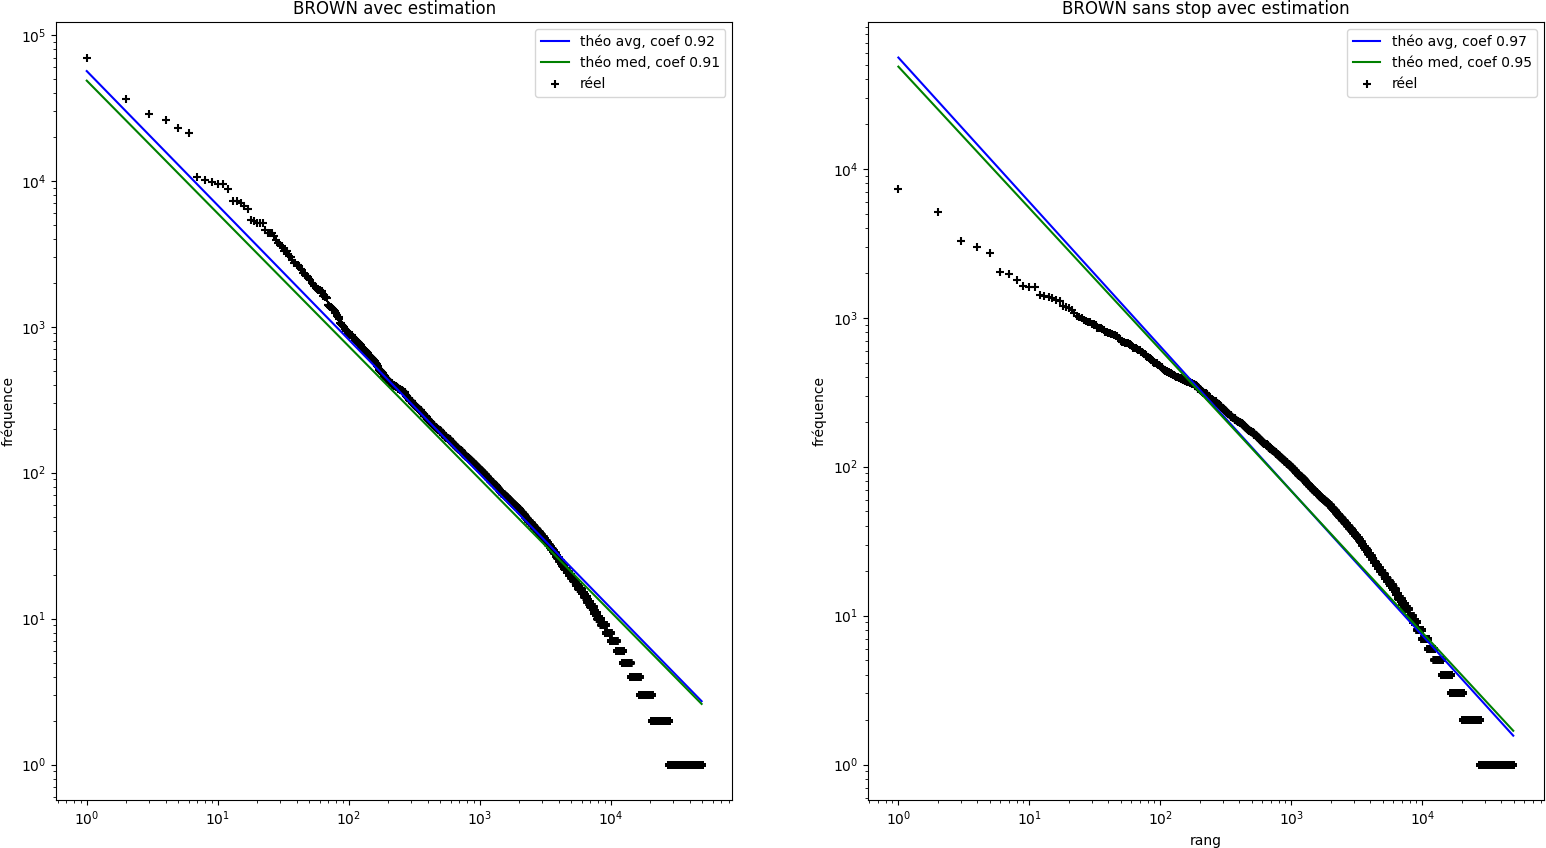
\includegraphics[width=\linewidth]{img/zipfFin.png}
			\caption{Distribution de Zipf avec les estimations}
		\end{figure}
		
		En conclusion, j'utiliserais la moyenne des constantes sur un document complet afin de déterminer le coefficient dans ma recherche de spam. 
		
		\subparagraph{Notes:}
			L'ensemble des codes sources pour cette partie est disponible dans les fichiers :
			\begin{itemize}
				\item[•]./analyse/rech\_zipf.py
				\item[•] ./traitement/stats.py
			\end{itemize}
		


\newpage
\section{Tableau des choix technologiques}
	\begin{tabular}{|p{3cm}|c|p{4cm}|p{6cm}|}
		\hline
		Élément & Retenu & Raisons & Observations \\
		\hline
		
		\multicolumn{4}{|c|}{Datasets} \\
		\hline
		Mail de la compagnie Enron & Non & Mails non classés & Non retenu pour la phase de développement car pas de moyen fiable de contrôler la sortie automatiquement \\
		\hline
		Mail du projet SpamAssassin & Oui & Mails déjà pré-triés & Mails principalement en Anglais déjà pré-trié en catégorie Spam et Ham \\
		\hline
		Brown dataset (nltk) & Oui & Corpus d'un million de mots en Anglais publié en 1961 & Dataset utilisé pour le développement de la visualisation de la distribution de Zipf\\
		\hline
		Stopwords (nltk) & Oui & Corpus de mots commun non significatif dans un texte & Utilisation dans le développement de la visualisation de la distribution de Zipf\\
		\hline
		
		\multicolumn{4}{|c|}{Langage et Modules} \\
		\hline
		Python & Oui & Langage polyvalent pour le traitement des données & \\		
		\hline
		Module email & Oui & Module natif pour le traitement des mails & Grande flexibilité pour la lecture des mails \\
		\hline
				
		\multicolumn{4}{|c|}{Bases de données} \\
		\hline
		ElasticSearch & Oui & Technologie utilisée dans mon entreprise. Présence d'une interface de visualisation des données Kibana. & Application dockerisée. \\
		\hline
		PostgreSQL & Oui & Moteur de base de données relationnelle plus facilement scalable que ElasticSearch pour l'ajout de nouvelle catégorie de données. Il n'est pas nécessaire de ré-indexer toute la base pour ajouter des champs & Application dockerisée\\
		\hline
		SQLite & Oui & Base de données légère pour stocker uniquement les données statistiques des étapes de la phase 1 & Rapide à mettre en place et déjà intégrée \\
		\hline		
		
		\hline
	\end{tabular}
	
	\section{Modèles}	
		\subsection{Naive Bayes}
	
	\section{Bibliographie}
	
	\section{Sitotec}
		\subsection{Corpus}
			\begin{itemize}
				\item Enron company mails, fichier CSV contenant l'ensemble des mails d'une entreprise ayant fermée ses portes (33.834.245 mails) [en ligne], \url{https://www.kaggle.com/wcukierski/enron-email-dataset} (consulté le 27/01/2022) \label{Enron_dataset}
				\item Mails project SpamAssassin, projet opensource de détection de spam (6065 fichiers email déjà trier en ham et spam) [en ligne], \url{https://spamassassin.apache.org/old/publiccorpus/} (consulté le 27/01/2022) \label{SpamAssassin_dataset}
				\item Brown corpus, ensemble de texte en anglais publié en 1961 qui contient plus d'un million de mots \url{https://www.nltk.org/book/ch02.html} (consulté le 20/08/2022) \label{Brown_corpus}
			\end{itemize}
		
		\subsection{Sites}
			\paragraph{Module langdetect}
			\begin{itemize}
				\item Page Github du projet \emph{langdetect} capable de différencier 49 langages avec une précision de 99\%, [en ligne] \url{https://github.com/Mimino666/langdetect} (consulté le 04/12/2022) \label{langdetect}
				\item Language Detection Library, présentation du module (anglais) [en ligne] \url{https://www.slideshare.net/shuyo/language-detection-library-for-java} (consulté le 04/12/2022)
			\end{itemize}
		
		

\end{document}




	\section{math}
		\paragraph{Equation avec fraction}
			\begin{eqnarray*}
				x\cdot\left(1-\frac{75}{100}\right) &=& 50\\
				x \cdot \frac{25}{100} &=& 50\\
				x &=& 50 \cdot \frac{100}{25}\\
				x &=& \sqrt{200}
			\end{eqnarray*}
		\paragraph{Equation dans texte}
			Sur ce dessin, on dispose un point M tel que $AM = BM$
	
	\section{Image}
		On peut aussi montrer les choses en image. Dans ce cas, il ne faut jamais oublier de mettre une légende et de citer ses sources si on a piqué l'image quelque part (cf: Figure \textcolor{blue}{1}) :
		\begin{figure}[h]
			\begin{center}
				\includegraphics[scale=0.2]{ProblemSolving.eps} % Le scale est peut être un peu petit.
			\end{center}
			\caption{Un graphe amusant sur la résolution de problème proposé comme exemple par le logiciel YeD.}
		\end{figure}
		
		\begin{figure}[H]
  			\includegraphics[width=\linewidth]{boat.jpg}
  			\caption{A boat.}
  			\label{fig:boat1}
		\end{figure}
		
		Figure \ref{fig:boat1} shows a boat.
		
		\begin{figure}[h!]
  			\centering
  				\begin{subfigure}[b]{0.4\linewidth}
    				\includegraphics[width=\linewidth]{coffee.jpg}
    				\caption{Coffee.}
  				\end{subfigure}
  				\begin{subfigure}[b]{0.4\linewidth}
    				\includegraphics[width=\linewidth]{coffee.jpg}
    				\caption{More coffee.}
  				\end{subfigure}
  				\caption{The same cup of coffee. Two times.}
  				\label{fig:coffee}
		\end{figure}	
		
		
	
	\section{Tableau}
		\begin{itemize}
			\item on énumère différents éléments,
			\item chacun sur une ligne,
			\item séparés par des virgules,
			\item et précédés d'une puce mettant en valeur l'énumération.
		\end{itemize}
	
		\begin{tabular}{|c|l|c|c|}
			\hline
			\multicolumn{4}{|c|}{Résolution de problème} \\
			\hline
			étape & description & si oui aller à & sinon aller à \\
			\hline
			A & Est-ce que ça marche  & B & C \\
			\hline
			B & N'y touche pas !! & \multicolumn{2}{|c|}{K} \\
			\hline
			C & Est-ce que tu y as touché ? & D & H \\
			\hline
			D & Espèce d'idiot !!! & \multicolumn{2}{|c|}{E} \\
			\hline
			E & Est-ce que quelqu'un le sait ? & F & G \\
			\hline
			F & T'es vraiment un pauvre idiot ! & \multicolumn{2}{|c|}{G} \\
			\hline
			G & Est-que tu peux imputer la faute à quelqu'un d'autre ? & K & F \\
			\hline
			H & Est-ce que ça va te pourrir la vie ? & F & I \\
			\hline
			I & Jette le et n'y pense plus !! & \multicolumn{2}{|c|}{K} \\
			\hline
			J & Cache le !! & \multicolumn{2}{|c|}{K} \\
			\hline
			K & Y'a pas de problème !! & & \\
			\hline
		\end{tabular}
		
		\section{Liste à puces}

	Une liste à puce se présente de cette manière :

	\begin{itemize}
		\item on énumère différents éléments,
		\item chacun sur une ligne,
		\item séparés par des virgules,
		\item et précédés d'une puce mettant en valeur l'énumération.
	\end{itemize}

\section{Liste numérotée}

	Une énumération est assez similaire :
	
	\begin{enumerate}
		\item une fois de plus,
		\item les éléments sont isolés chacun sur une ligne.
		\item La différence notable est que chaque élément est numéroté,
		\item ce qui permet de mettre en valeur sont rang,
		\item ou bien de faciliter le compte du nombre total d'éléments.
	\end{enumerate}
	
\section{Code}
	\begin{verbatim}
	
	\end{verbatim}
	
	\begin{verbatimtab}[2]
	
	\end{verbatimtab}
		
	\begin{lstlisting}
#!/usr/bin/perl
print S(@ARGV);sub S{$r=(@_[0]%4==0&&@_[0]%100!=0)||@_[0]%400=0;}
	\end{lstlisting}
	
	\lstinputlisting[caption={TITRE}, language=c]{script.pl}
	
\section{quote}
	\begin{displayquote}
Sé que tengo un ego del tamaño de un planeta pequeño, pero incluso yo a 
veces me equivoco
	\end{displayquote}